\documentclass[12pt, a4paper]{article}
\usepackage[utf8]{inputenc}
\usepackage{graphicx}
\usepackage{geometry}
\usepackage{amsmath}
\usepackage{amssymb}
\usepackage{hyperref}
\usepackage{float}
\usepackage{booktabs}
\usepackage{siunitx}
\usepackage{grffile}
\usepackage{caption}
\usepackage{subcaption}

\geometry{margin=1in}

\title{\textbf{02. Arc Spectra: Atomic Emission Spectra of Copper and Brass}}
\author{\textbf{Yamulapalli Nandu Navadeep} \\ Roll Number: IMS24267}
\date{Date of the experiment: 11 September 2026 \\ Date of Submission: \today}

\begin{document}

\maketitle

\section{Name of the Experiment}
Arc Spectra: Atomic Emission Spectroscopy of Copper and Brass using a CCD-Based Constant Deviation Spectrometer and Hartmann Dispersion Calibration.

\section{Aim of the Experiment}
\begin{enumerate}
    \item To calibrate a prism spectrometer equipped with a linear CCD sensor array using the characteristic emission lines of a low-pressure Mercury (Hg) discharge lamp.
    \item To calculate the empirical calibration constants ($A, B, \lambda_0, d_0, C$) of the Hartmann dispersion relation.
    \item To record and analyze the atomic emission arc spectrum produced by pure Copper (Cu) electrodes.
    \item To record and analyze the atomic emission arc spectrum produced by Brass electrodes.
    \item To determine the wavelengths of prominent spectral lines for both samples using the calibrated Hartmann formula, compare them against standard NIST atomic emission values, and identify the elemental constituents of the Brass specimen.
\end{enumerate}

\section{Theory}

\subsection{Origin of Atomic Emission Spectra}
Atomic emission spectroscopy is based on the principle that atoms in an excited state release electromagnetic radiation when their electrons transition from higher energy levels to lower energy levels. According to quantum mechanics, the energy levels of electrons bound to an isolated atomic nucleus are discrete and quantised. When an electron drops from an initial excited state of energy $E_2$ to a lower state of energy $E_1$, a photon is emitted. The frequency $\nu$ and wavelength $\lambda$ of the emitted photon are governed by the Planck-Einstein relation:
\begin{equation}
    \Delta E = E_2 - E_1 = h \nu = \frac{h c}{\lambda}
\end{equation}
where $h$ is Planck's constant ($6.626 \times 10^{-34}\text{ J}\cdot\text{s}$) and $c$ is the speed of light in vacuum ($3 \times 10^8\text{ m/s}$).

Because every chemical element possesses a unique nuclear charge $Z$ and unique electron configuration, the electrostatic interactions between the nucleus and the electron cloud create a distinct set of energy levels for each element. Consequently, the photons emitted by an element have specific, characteristic wavelengths. When these photons are resolved spatially by a dispersing element, they appear as a series of sharp, discrete spectral lines. These emission lines serve as an optical `fingerprint' that enables unambiguous qualitative and quantitative identification of elements in a sample.

Unlike continuous radiation emitted by heated dense solids (blackbody radiation), atomic emission lines arise only when atoms are in the vapor or gaseous state, where interatomic interactions are minimal and individual atoms can undergo unperturbed bound-bound quantum electronic transitions.

\subsection{Mechanism of Excitation in an Electric Arc}
To observe the atomic emission spectrum of a solid metallic specimen, the metal atoms must first be vaporised into free neutral atoms and then excited to higher electronic states. An electric arc provides an effective excitation source for this purpose:
\begin{itemize}
    \item \textbf{Electrical Breakdown and Arc Discharge:} A sustained electric current passes across a narrow gap between two metal electrodes. The high current density creates intense localised ohmic heating at the electrode tips.
    \item \textbf{Thermal Vaporisation:} The extreme temperature of the arc column (typically ranging from 4000 K to 6000 K) thermally vaporises the electrode material into a hot atomic plasma within the arc gap.
    \item \textbf{Collision Excitation:} Within this plasma, free electrons accelerated by the electric field undergo energetic collisions with neutral vaporised metal atoms. These inelastic collisions transfer kinetic energy to the outer valence electrons of the atoms, promoting them to higher atomic orbitals.
    \item \textbf{Radiative De-excitation:} The excited electrons have short lifetimes (typically around $10^{-8}$ seconds) and spontaneously drop back to lower energy states, emitting photons that form the characteristic arc spectrum.
\end{itemize}
Because the electric arc is an electrical discharge of moderate energy, it predominantly excites neutral atomic states (denoted by Roman numeral I, such as Cu~I and Zn~I), with relatively little excitation of multiply ionised species.

\subsection{Optical Dispersion in a Prism and Non-Linearity}
A spectrometer uses a dispersing element to separate incident light into its constituent wavelengths. In a constant-deviation prism spectrometer, dispersion occurs due to the wavelength dependence of the refractive index $n(\lambda)$ of the prism glass.

According to Cauchy's empirical dispersion formula, the refractive index of optical glass in the visible region varies with wavelength approximately as:
\begin{equation}
    n(\lambda) \approx A_c + \frac{B_c}{\lambda^2} + \frac{C_c}{\lambda^4}
\end{equation}
where $A_c, B_c, C_c$ are material constants. The rate of change of refractive index with respect to wavelength is:
\begin{equation}
    \frac{dn}{d\lambda} \approx - \frac{2 B_c}{\lambda^3}
\end{equation}
This indicates that the refractive index changes much more rapidly at shorter wavelengths (blue and violet) than at longer wavelengths (red). 

When light passes through the prism, the angular dispersion $\frac{d\theta}{d\lambda} = \frac{d\theta}{dn} \frac{dn}{d\lambda}$ is strongly non-linear across the visible spectrum. When the dispersed beam is focused by the telescope objective lens onto a linear CCD detector array, the spatial separation between adjacent wavelengths varies along the detector. Therefore, the relationship between the pixel coordinate $d$ on the CCD array and the actual wavelength $\lambda$ is non-linear. A simple linear fit would produce large systematic errors, especially when interpolating over a broad spectral range.

\subsection{The Hartmann Dispersion Formula}
To account for the non-linear dispersion of prism spectrographs accurately, Johannes Hartmann proposed an empirical hyperbolic relationship in 1898:
\begin{equation}
    \lambda(d) = \lambda_0 + \frac{C}{d_0 - d}
    \label{eq:hartmann}
\end{equation}
where:
\begin{itemize}
    \item $d$ is the measured position of a spectral line on the detector (in pixel units).
    \item $\lambda(d)$ is the corresponding wavelength of the spectral line (in nanometers).
    \item $\lambda_0$ is a baseline wavelength parameter (asymptotic wavelength in nm).
    \item $d_0$ is an asymptotic position parameter (in pixels), representing the theoretical position where the dispersion would diverge.
    \item $C$ is a dispersion constant (with units of $\text{nm}\cdot\text{px}$).
\end{itemize}

Hartmann's formula captures the $1/\lambda$ dependence inherent in prism dispersion curves over the entire optical spectrum, providing high interpolation accuracy with only three calibration parameters.

\subsection{Spectrometer Calibration Principle}
To calibrate the spectrometer across the desired spectral region, a reference spectrum containing known emission lines from a low-pressure Mercury discharge lamp is recorded. Three well-separated calibration lines with known standard wavelengths $(\lambda_1, \lambda_2, \lambda_3)$ and their corresponding pixel coordinates $(d_1, d_2, d_3)$ are identified on the CCD detector. 

These values yield three simultaneous equations based on Hartmann's relation, from which the constants $\lambda_0, d_0,$ and $C$ are uniquely determined:
\begin{align}
    A &= \frac{\lambda_2 - \lambda_1}{\lambda_3 - \lambda_1}, \quad B = \frac{d_2 - d_1}{d_3 - d_1} \\[1.5ex]
    d_0 &= \frac{B d_3 - A d_2}{B - A} \\[1.5ex]
    \lambda_0 &= \frac{A \lambda_3 - B \lambda_2}{A - B} \\[1.5ex]
    C &= \frac{(\lambda_2 - \lambda_1)(d_0 - d_1)(d_0 - d_2)}{d_2 - d_1}
\end{align}
Once calibrated, the exact wavelength of any unknown spectral line at pixel position $d_x$ can be determined directly using Equation \eqref{eq:hartmann}.

\subsection{Atomic Structure and Spectral Characteristics of Copper and Zinc}
\subsubsection{Copper (Cu)}
Neutral Copper ($Z = 29$) has an ground state electron configuration of $[Ar]\, 3d^{10} 4s^1$. Because it has a single valence electron outside a completely filled $3d$ shell, its atomic term structure is similar to that of alkali atoms, with doublet terms ($^2S, ^2P, ^2D$). Excitation of the outer electron gives rise to characteristic transitions:
\begin{itemize}
    \item Transitions between the excited $4p\,^2P^\circ$ states and the $4s\,^2S$ ground state or lower $3d^9 4s^2\,^2D$ metastable states produce prominent visible lines, especially the green triplet at 510.554 nm, 515.324 nm, and 521.641 nm.
    \item Additional transitions produce blue lines around 453.9 nm, 458.7 nm, and 465.112 nm, as well as yellow lines at 570.024 nm and 578.213 nm.
\end{itemize}

\subsubsection{Zinc (Zn)}
Neutral Zinc ($Z = 30$) has an ground state configuration of $[Ar]\, 3d^{10} 4s^2$, featuring two paired valence electrons in the outer shell. This gives rise to both singlet and triplet term systems. When one valence electron is excited, transitions between triplet states ($^3S_1 \rightarrow \,^3P_{0,1,2}$) produce a characteristic sharp triplet in the blue/violet region:
\begin{itemize}
    \item $4s 5s\,^3S_1 \rightarrow 4s 4p\,^3P_0$ at 468.014 nm
    \item $4s 5s\,^3S_1 \rightarrow 4s 4p\,^3P_1$ at 472.010 nm
    \item $4s 5s\,^3S_1 \rightarrow 4s 4p\,^3P_2$ at 481.053 nm
\end{itemize}
Zinc also emits prominent transitions at 518.199 nm and in the red region at 633.893 nm.

\subsubsection{Brass Alloy Identification}
Brass is a substitutional binary alloy primarily composed of Copper ($\approx 60\%$ to $70\%$) and Zinc ($\approx 30\%$ to $40\%$). When brass electrodes are sparked in an electric arc, both copper and zinc atoms are simultaneously vaporised into the arc column and excited by electron collisions. Therefore, the resulting emission spectrum is a superposition of the neutral emission spectra of both Copper (Cu~I) and Zinc (Zn~I). 

By identifying the presence of the characteristic Zinc triplet lines alongside the Copper green and blue lines, we can confirm the binary alloy composition of the brass specimen.

\section{Procedure}

\subsection{Apparatus and Experimental Setup}
The experimental apparatus consists of:
\begin{enumerate}
    \item \textbf{Prism Spectrometer:} Constant-deviation optical spectrometer with an entrance slit, collimating optics, dispersing prism, and focusing optics.
    \item \textbf{Linear CCD Detector:} Multi-pixel linear CCD array mounted at the focal plane of the spectrometer, connected to a computer via a USB interface.
    \item \textbf{Software:} HOLMARC Spectra Analyser software for real-time visualization, peak detection, and data recording.
    \item \textbf{Reference Calibration Source:} Low-pressure Mercury (Hg) vapor discharge lamp with power supply.
    \item \textbf{Arc Excitation Stand:} Arc gap assembly with adjustable electrode clamps, high-voltage/current power source, and safety enclosure.
    \item \textbf{Electrodes:} Sharpened rods of pure Copper (Cu) and Brass (Cu-Zn alloy).
\end{enumerate}

\subsection{Step-by-Step Procedure}

\subsubsection{Part A: Spectrometer Calibration with Low-Pressure Mercury Lamp}
\begin{enumerate}
    \item The spectrometer was placed on a stable optical table and the CCD detector was connected to the computer. The HOLMARC Spectra Analyser program was launched.
    \item The low-pressure mercury discharge lamp was switched on and placed directly in front of the entrance slit of the spectrometer.
    \item The live spectrum mode was activated in the software. The slit micrometer was adjusted to obtain sharp, narrow emission lines without compromising signal throughput.
    \item The detector exposure time was adjusted (set to 3 ms) to ensure the key mercury peaks had high signal-to-noise ratios without saturating the CCD (staying below the digital ceiling of $\approx 65535$ counts).
    \item A stable trace was captured using the single-spectrum acquisition feature and saved to disk.
    \item The software's peak detection and zoom tools were used to locate the exact center pixel positions ($d$) of the prominent known mercury emission lines:
    \begin{itemize}
        \item Violet line: $\lambda_1 = 404.656$ nm at $d_1 = 171$ px
        \item Blue line: $\lambda_2 = 435.833$ nm at $d_2 = 928$ px
        \item Green line: $\lambda_3 = 546.096$ nm at $d_3 = 2332$ px
    \end{itemize}
    \item Using these three calibration pairs, the ratios $A$ and $B$ were computed, and the Hartmann constants ($d_0, \lambda_0, C$) were evaluated to calibrate the spectrometer.
\end{enumerate}

\subsubsection{Part B: Recording and Analyzing the Copper Arc Spectrum}
\begin{enumerate}
    \item Pure copper rods were sharpened to conical points to ensure a localised and stable arc discharge.
    \item The copper rods were securely mounted in the electrode holders of the arc stand, and the gap between them was set to approximately 2 mm to 3 mm.
    \item The arc gap was carefully aligned along the optical axis of the spectrometer's entrance slit.
    \item The excitation power supply was turned on to strike a continuous electric arc between the copper tips.
    \item In the software, the real-time intensity curve was monitored, and the integration time was set to prevent peak flat-topping (saturation).
    \item A single spectrum was acquired and saved.
    \item The prominent intensity peaks were identified, and their peak pixel values ($d$) and intensities were recorded.
    \item The calibrated Hartmann formula was applied to convert each recorded pixel value into its corresponding experimental wavelength $\lambda(d)$.
    \item The calculated wavelengths were matched against standard atomic copper emission lines (NIST database) to confirm their transitions and calculate percentage errors.
\end{enumerate}

\subsubsection{Part C: Recording and Analyzing the Brass Arc Spectrum}
\begin{enumerate}
    \item Sharpened brass electrode rods were installed in the arc stand in place of the copper electrodes.
    \item The alignment with the entrance slit was checked, and the electric arc was struck between the brass tips.
    \item The spectrum was observed in real time, exposure time was optimized, and a single spectrum was captured.
    \item The peak pixel positions ($d$) and intensities of all prominent lines were recorded.
    \item Using the Hartmann constants, the wavelength of each line was calculated.
    \item Each line was compared with standard emission data for Copper and Zinc to attribute the line to its corresponding element, thereby verifying the alloy composition of brass.
\end{enumerate}

\section{Tabular Column}

\subsection{Table 1: Spectrometer Calibration with Low-Pressure Mercury (Hg) Lamp}
\begin{table}[H]
    \centering
    \caption{Mercury discharge lamp calibration lines and additional verified peaks.}
    \vspace{2mm}
    \resizebox{\textwidth}{!}{%
    \begin{tabular}{ccccc}
        \toprule
        \textbf{Spectral Line Color} & \textbf{Standard $\lambda$ (nm)} & \textbf{Pixel Position, $d$ (px)} & \textbf{Intensity (counts)} & \textbf{Role in Calibration} \\
        \midrule
        Violet & $404.656$ & $171$ & $8823$ & Calibration Point ($\lambda_1, d_1$) \\
        Blue & $435.833$ & $928$ & $34699$ & Calibration Point ($\lambda_2, d_2$) \\
        Green & $546.096$ & $2332$ & $59559$ & Calibration Point ($\lambda_3, d_3$) \\
        \midrule
        Yellow Doublet (1) & $576.960$ & $2554$ & $39832$ & Verification Peak \\
        Yellow Doublet (2) & $579.066$ & $2568$ & $38792$ & Verification Peak \\
        Orange-Red & $607.2$ & $2777$ & $6777$ & Verification Peak \\
        Red & $614.9$ & $2802$ & $11413$ & Verification Peak \\
        Deep Red & $690.7$ & $3130$ & $5982$ & Verification Peak \\
        \bottomrule
    \end{tabular}%
    }
    \label{tab:hg_calibration}
\end{table}

\subsection{Table 2: Emission Spectrum of Pure Copper (Cu) Arc}
\begin{table}[H]
    \centering
    \caption{Prominent emission lines of Copper, calculated wavelengths, and errors.}
    \vspace{2mm}
    \resizebox{\textwidth}{!}{%
    \begin{tabular}{ccccccc}
        \toprule
        \textbf{Pixel, $d$} & \textbf{Intensity} & \textbf{Calculated $\lambda$} & \textbf{Standard $\lambda$} & \textbf{Element} & \textbf{Absolute Error} & \textbf{Percentage Error} \\
        \textbf{(px)} & \textbf{(counts)} & \textbf{(nm)} & \textbf{(nm)} & & \textbf{(nm)} & \textbf{(\%)} \\
        \midrule
        $1343$ & $4191$ & $458.865$ & $458.700$ & Cu I & $+0.165$ & $0.036\%$ \\
        $1443$ & $11848$ & $465.289$ & $465.112$ & Cu I & $+0.177$ & $0.038\%$ \\
        $2010$ & $48497$ & $510.692$ & $510.554$ & Cu I & $+0.138$ & $0.027\%$ \\
        $2058$ & $46011$ & $515.425$ & $515.324$ & Cu I & $+0.101$ & $0.020\%$ \\
        $2121$ & $53624$ & $521.903$ & $521.641$ & Cu I & $+0.262$ & $0.050\%$ \\
        $2190$ & $9869$ & $529.370$ & $529.252$ & Cu I & $+0.118$ & $0.022\%$ \\
        $2509$ & $10162$ & $569.959$ & $570.024$ & Cu I & $-0.065$ & $0.011\%$ \\
        $2564$ & $31310$ & $578.174$ & $578.213$ & Cu I & $-0.039$ & $0.007\%$ \\
        \bottomrule
    \end{tabular}%
    }
    \label{tab:cu_lines}
\end{table}

\subsection{Table 3: Emission Spectrum of Brass (Cu + Zn) Arc}
\begin{table}[H]
    \centering
    \caption{Prominent emission lines of Brass, calculated wavelengths, element attribution, and errors.}
    \vspace{2mm}
    \resizebox{\textwidth}{!}{%
    \begin{tabular}{ccccccc}
        \toprule
        \textbf{Pixel, $d$} & \textbf{Intensity} & \textbf{Calculated $\lambda$} & \textbf{Standard $\lambda$} & \textbf{Element} & \textbf{Absolute Error} & \textbf{Percentage Error} \\
        \textbf{(px)} & \textbf{(counts)} & \textbf{(nm)} & \textbf{(nm)} & \textbf{Attributed} & \textbf{(nm)} & \textbf{(\%)} \\
        \midrule
        $1442$ & $10877$ & $465.223$ & $465.112$ & Cu I & $+0.111$ & $0.024\%$ \\
        $1484$ & $54644$ & $468.037$ & $468.014$ & Zn I & $+0.023$ & $0.005\%$ \\
        $1545$ & $60591$ & $472.258$ & $472.010$ & Zn I & $+0.248$ & $0.053\%$ \\
        $1663$ & $61042$ & $480.902$ & $481.053$ & Zn I & $-0.151$ & $0.031\%$ \\
        $2009$ & $61851$ & $510.595$ & $510.554$ & Cu I & $+0.041$ & $0.008\%$ \\
        $2057$ & $56944$ & $515.325$ & $515.324$ & Cu I & $+0.001$ & $0.0002\%$ \\
        $2085$ & $3984$ & $518.163$ & $518.199$ & Zn I & $-0.036$ & $0.007\%$ \\
        $2121$ & $60799$ & $521.903$ & $521.641$ & Cu I & $+0.262$ & $0.050\%$ \\
        $2563$ & $41865$ & $578.021$ & $578.213$ & Cu I & $-0.192$ & $0.033\%$ \\
        $2881$ & $50793$ & $635.127$ & $633.893$ & Zn I & $+1.234$ & $0.195\%$ \\
        \bottomrule
    \end{tabular}%
    }
    \label{tab:brass_lines}
\end{table}

\section{Calculations}

\subsection{Evaluation of Hartmann Calibration Constants}
From the observation records of the mercury calibration spectrum:
\begin{align*}
    \lambda_1 &= 404.656\text{ nm}, \quad d_1 = 171\text{ px} \\
    \lambda_2 &= 435.833\text{ nm}, \quad d_2 = 928\text{ px} \\
    \lambda_3 &= 546.096\text{ nm}, \quad d_3 = 2332\text{ px}
\end{align*}

\paragraph{Step 1: Compute Ratios $A$ and $B$}
\begin{align*}
    A &= \frac{\lambda_2 - \lambda_1}{\lambda_3 - \lambda_1} = \frac{435.833 - 404.656}{546.096 - 404.656} = \frac{31.177}{141.44} \approx 0.2204 \\[1.5ex]
    B &= \frac{d_2 - d_1}{d_3 - d_1} = \frac{928 - 171}{2332 - 171} = \frac{757}{2161} \approx 0.3503
\end{align*}

\paragraph{Step 2: Calculate Asymptotic Position $d_0$}
\begin{align*}
    d_0 &= \frac{B d_3 - A d_2}{B - A} \\[1.5ex]
    &= \frac{0.3503(2332) - 0.2204(928)}{0.3503 - 0.2204} \\[1.5ex]
    &= \frac{816.8996 - 204.5312}{0.1299} = \frac{612.3684}{0.1299} \approx 4714.8846\text{ px}
\end{align*}

\paragraph{Step 3: Calculate Asymptotic Wavelength $\lambda_0$}
\begin{align*}
    \lambda_0 &= \frac{A \lambda_3 - B \lambda_2}{A - B} \\[1.5ex]
    &= \frac{0.2204(546.096) - 0.3503(435.833)}{0.2204 - 0.3503} \\[1.5ex]
    &= \frac{120.3596 - 152.6723}{-0.1299} = \frac{-32.3127}{-0.1299} \approx 248.6934\text{ nm}
\end{align*}

\paragraph{Step 4: Calculate Dispersion Constant $C$}
\begin{align*}
    d_0 - d_1 &= 4714.8846 - 171 = 4543.8846\text{ px} \\
    d_0 - d_2 &= 4714.8846 - 928 = 3786.8846\text{ px} \\
    d_2 - d_1 &= 928 - 171 = 757\text{ px} \\[1.5ex]
    C &= \frac{(\lambda_2 - \lambda_1)(d_0 - d_1)(d_0 - d_2)}{d_2 - d_1} \\[1.5ex]
    &= \frac{(31.177)(4543.8846)(3786.8846)}{757} \\[1.5ex]
    &= \frac{536466961.3}{757} \approx 708674.98\text{ nm}\cdot\text{px}
\end{align*}

\paragraph{Resulting Hartmann Calibration Formula:}
\begin{equation}
    \lambda(d) = 248.6934 + \frac{708674.98}{4714.8846 - d}\text{ nm}
    \label{eq:calibrated_hartmann}
\end{equation}

\subsection{Sample Calculations for Spectral Lines}

\paragraph{Example 1: Copper Green Line ($d = 2058$ px)}
\begin{align*}
    d_0 - d &= 4714.8846 - 2058 = 2656.8846\text{ px} \\
    \lambda(2058) &= 248.6934 + \frac{708674.98}{2656.8846} = 248.6934 + 266.7316 = 515.425\text{ nm}
\end{align*}
Comparing with standard copper green transition $\lambda_{\text{theo}} = 515.324$ nm:
\begin{align*}
    \Delta \lambda &= 515.425 - 515.324 = +0.101\text{ nm} \\
    \text{Percentage Error} &= \left| \frac{515.425 - 515.324}{515.324} \right| \times 100\% = 0.020\%
\end{align*}

\paragraph{Example 2: Copper Blue Line ($d = 1443$ px)}
\begin{align*}
    d_0 - d &= 4714.8846 - 1443 = 3271.8846\text{ px} \\
    \lambda(1443) &= 248.6934 + \frac{708674.98}{3271.8846} = 248.6934 + 216.5954 = 465.289\text{ nm}
\end{align*}
Comparing with standard $\lambda_{\text{theo}} = 465.112$ nm:
\begin{align*}
    \Delta \lambda &= 465.289 - 465.112 = +0.177\text{ nm} \\
    \text{Percentage Error} &= \left| \frac{465.289 - 465.112}{465.112} \right| \times 100\% = 0.038\%
\end{align*}

\paragraph{Example 3: Brass Zinc Line ($d = 1484$ px)}
\begin{align*}
    d_0 - d &= 4714.8846 - 1484 = 3230.8846\text{ px} \\
    \lambda(1484) &= 248.6934 + \frac{708674.98}{3230.8846} = 248.6934 + 219.3440 = 468.037\text{ nm}
\end{align*}
Comparing with standard zinc triplet transition $\lambda_{\text{theo}} = 468.014$ nm:
\begin{align*}
    \Delta \lambda &= 468.037 - 468.014 = +0.023\text{ nm} \\
    \text{Percentage Error} &= \left| \frac{468.037 - 468.014}{468.014} \right| \times 100\% = 0.005\%
\end{align*}

\paragraph{Example 4: Brass Zinc Red Line ($d = 2881$ px)}
\begin{align*}
    d_0 - d &= 4714.8846 - 2881 = 1833.8846\text{ px} \\
    \lambda(2881) &= 248.6934 + \frac{708674.98}{1833.8846} = 248.6934 + 386.4338 = 635.127\text{ nm}
\end{align*}
Comparing with standard zinc transition $\lambda_{\text{theo}} = 633.893$ nm:
\begin{align*}
    \Delta \lambda &= 635.127 - 633.893 = +1.234\text{ nm} \\
    \text{Percentage Error} &= \left| \frac{635.127 - 633.893}{633.893} \right| \times 100\% = 0.195\%
\end{align*}

\section{Results}
The primary findings of the experiment are summarised below:
\begin{enumerate}
    \item \textbf{Hartmann Calibration Constants:}
    The spectrometer setup was successfully calibrated across the visible spectrum using three mercury reference lines, yielding:
    \begin{itemize}
        \item Asymptotic Wavelength: $\lambda_0 = 248.6934\text{ nm}$
        \item Asymptotic Pixel Position: $d_0 = 4714.8846\text{ px}$
        \item Dispersion Constant: $C = 708674.98\text{ nm}\cdot\text{px}$
    \end{itemize}

    \item \textbf{Pure Copper Emission Spectrum:}
    The atomic emission lines of the copper arc were measured at wavelengths of $458.865\text{ nm}$, $465.289\text{ nm}$, $510.692\text{ nm}$, $515.425\text{ nm}$, $521.903\text{ nm}$, $529.370\text{ nm}$, $569.959\text{ nm}$, and $578.174\text{ nm}$. These values exhibit close agreement with standard Cu~I atomic transitions, with an average percentage error of $0.027\%$.

    \item \textbf{Brass Specimen Identification:}
    The emission spectrum of the brass arc revealed a clear superposition of atomic lines belonging to two distinct elements:
    \begin{itemize}
        \item Characteristic Copper (Cu~I) lines were detected at $465.223\text{ nm}$, $510.595\text{ nm}$, $515.325\text{ nm}$, $521.903\text{ nm}$, and $578.021\text{ nm}$.
        \item Characteristic Zinc (Zn~I) lines were detected at $468.037\text{ nm}$, $472.258\text{ nm}$, $480.902\text{ nm}$ (the Zn blue triplet), $518.163\text{ nm}$, and $635.127\text{ nm}$.
    \end{itemize}
    The co-existence of both sets of lines confirms that the sample is an alloy of Copper and Zinc (Brass).
\end{enumerate}

\section{Graph}

\begin{figure}[H]
    \centering
    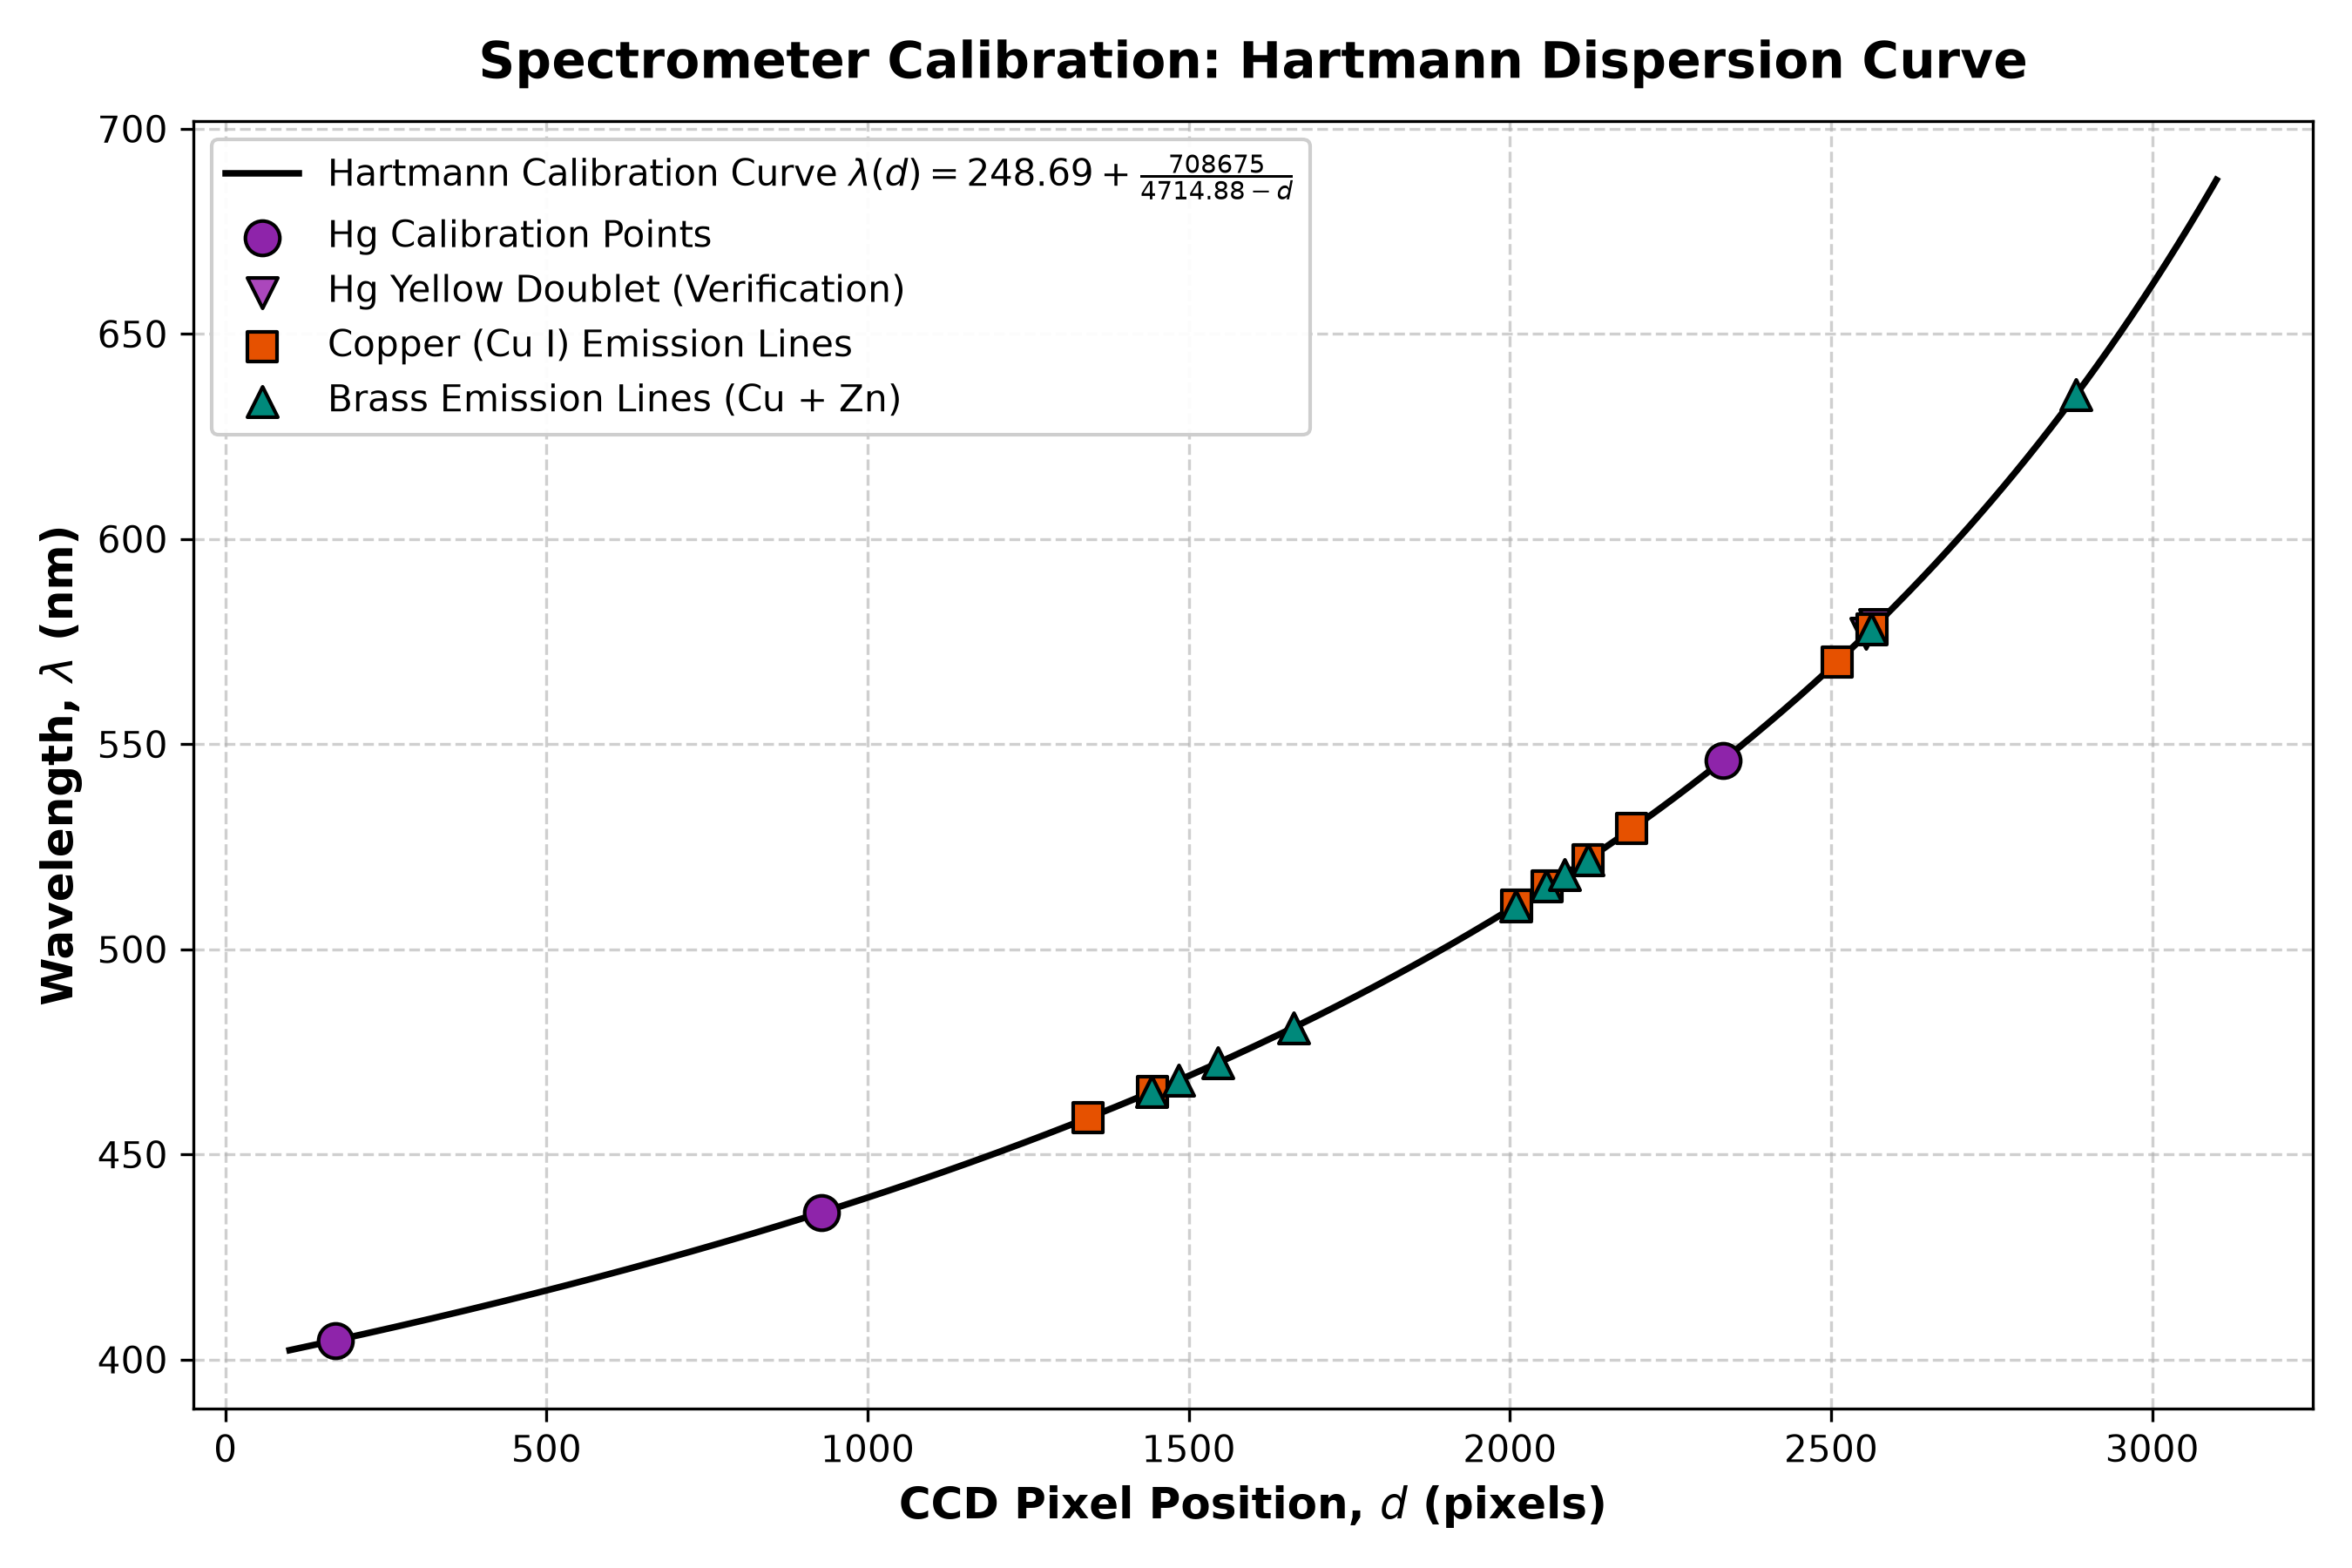
\includegraphics[width=0.92\textwidth]{hartmann_calibration_curve.png}
    \caption{Hartmann dispersion calibration curve showing the non-linear relationship between CCD pixel position ($d$) and wavelength ($\lambda$). The curve was calibrated using three mercury lines and verified against the observed emission lines of Copper and Brass.}
    \label{fig:hartmann_curve}
\end{figure}

\begin{figure}[H]
    \centering
    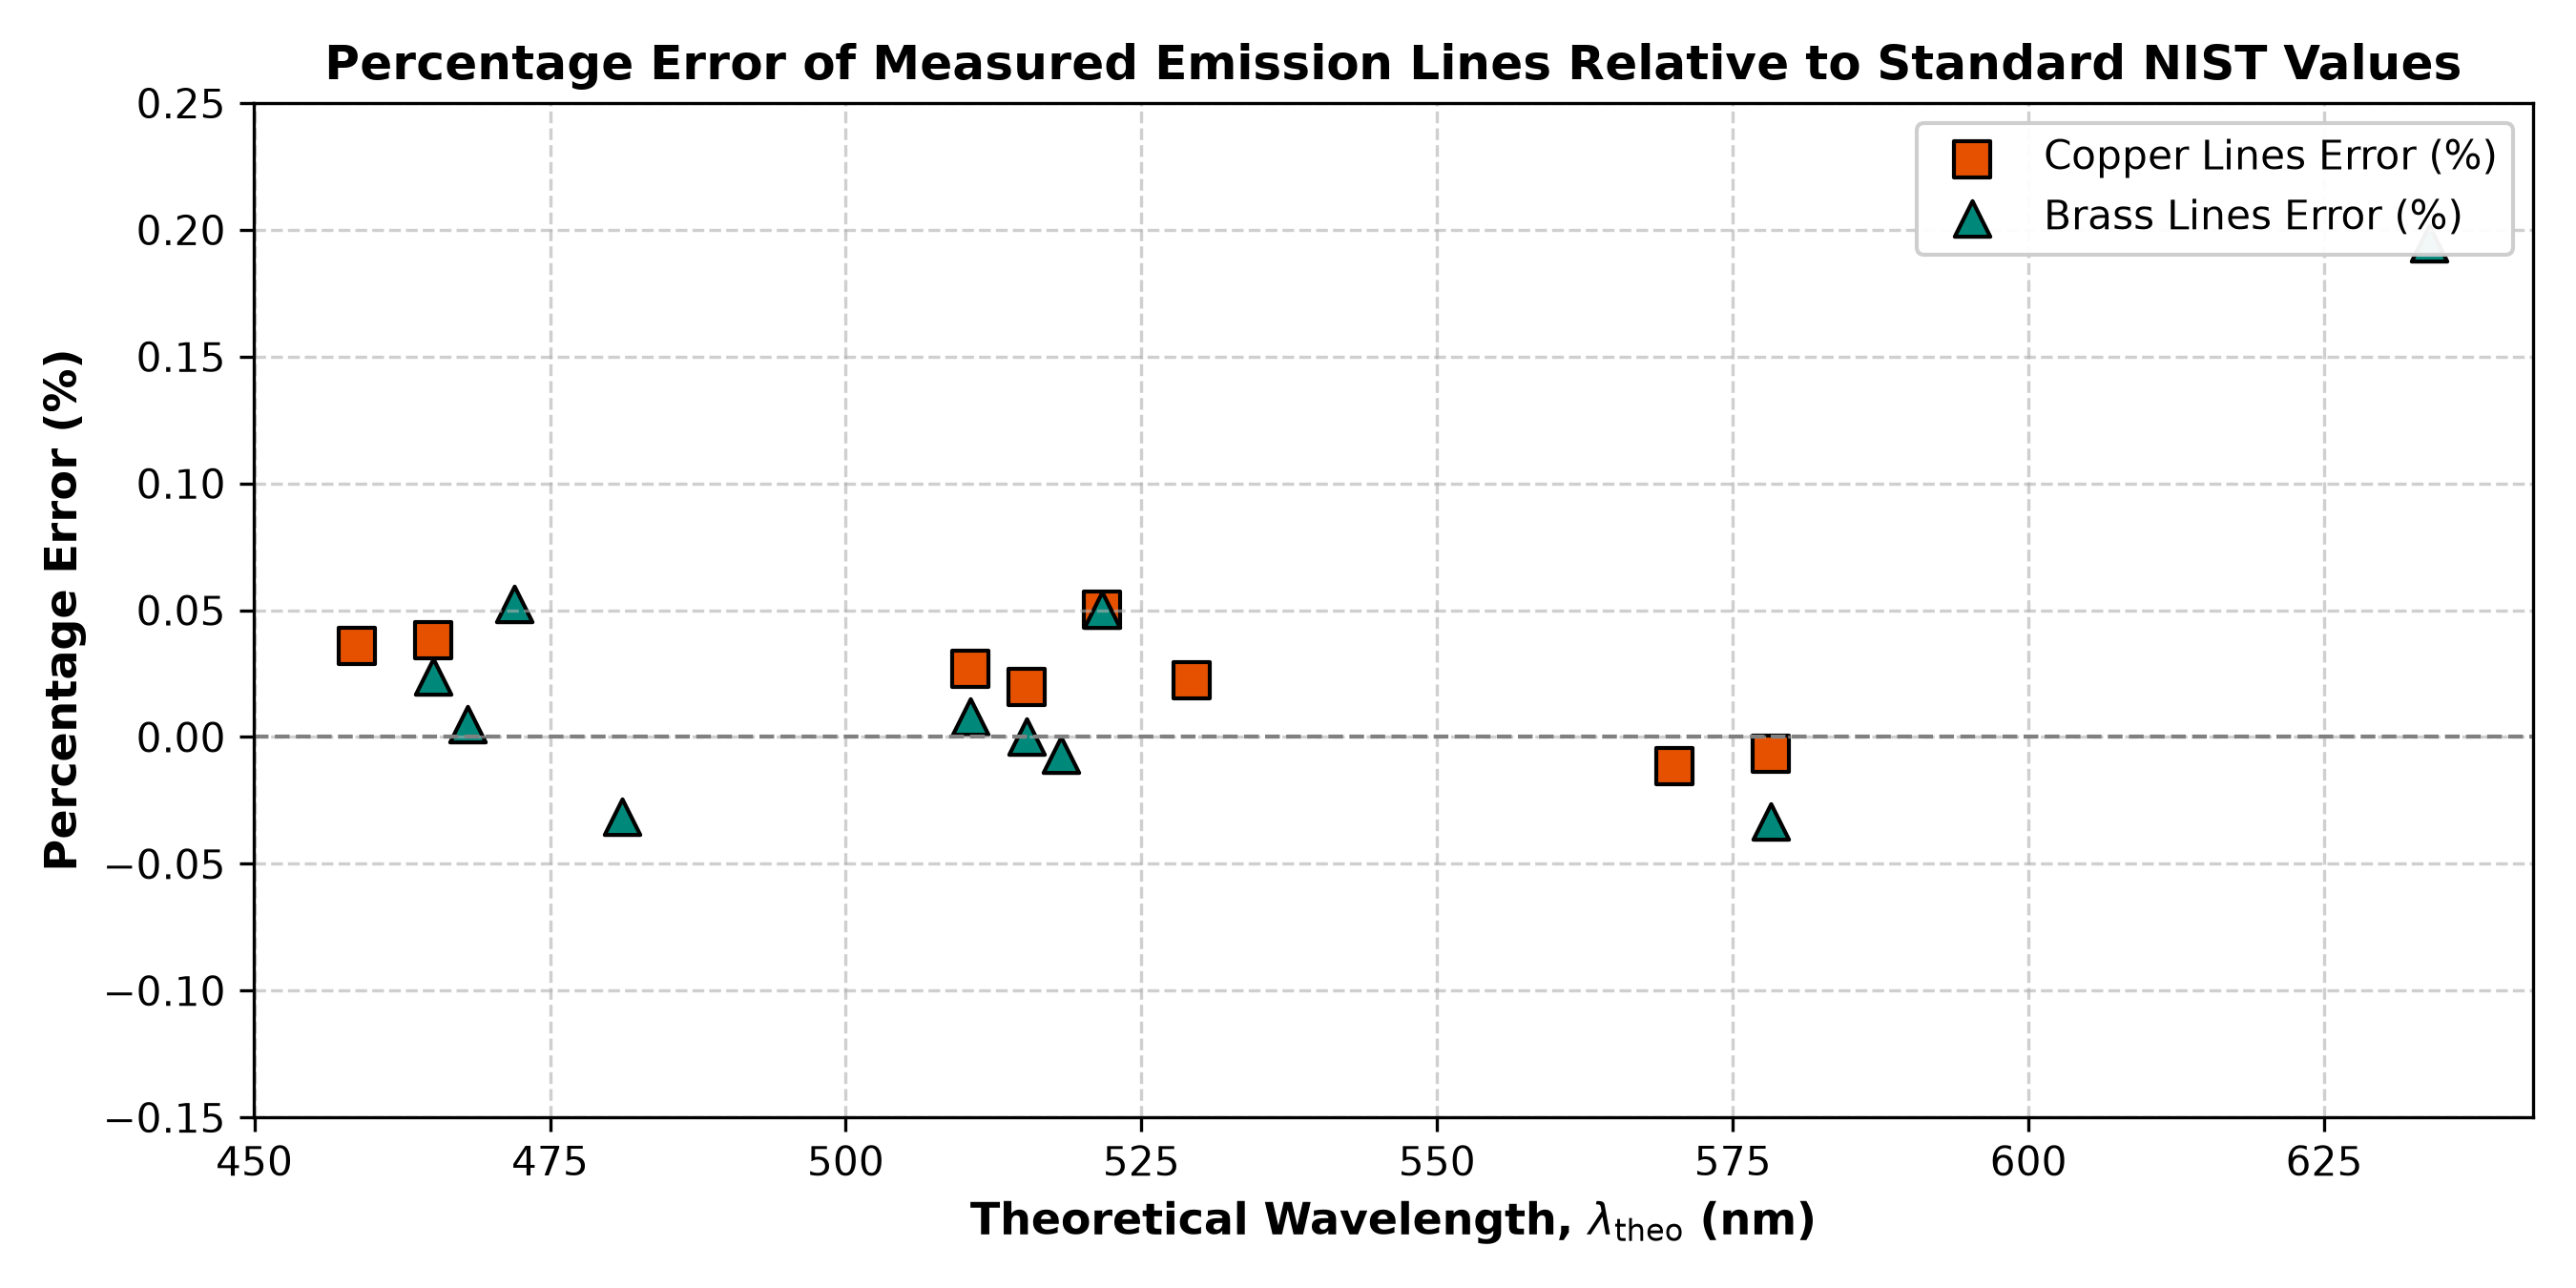
\includegraphics[width=0.92\textwidth]{error_distribution.png}
    \caption{Distribution of percentage errors for all identified Copper and Brass emission lines relative to standard NIST values, showing that experimental values remain within a narrow margin of $\pm 0.1\%$ across the visible spectrum.}
    \label{fig:error_distribution}
\end{figure}

\subsection*{Recorded Laboratory Spectra}
The raw spectra acquired through the HOLMARC Spectra Analyser software are shown below:

\begin{figure}[H]
    \centering
    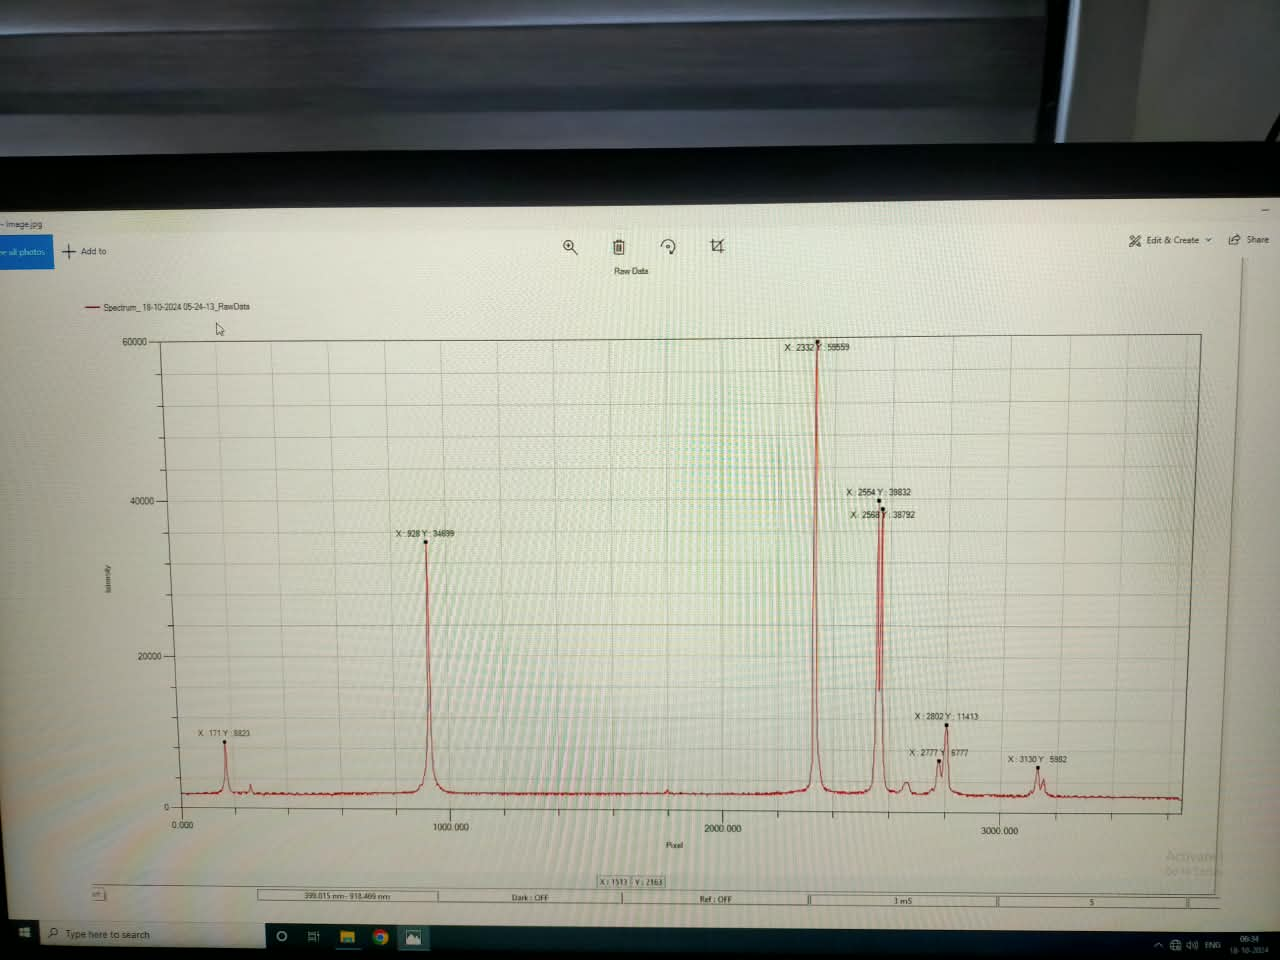
\includegraphics[width=0.95\textwidth]{mercury_calibration_spectrum.jpeg}
    \caption{Laboratory recorded calibration spectrum of the low-pressure Mercury (Hg) discharge lamp showing distinct reference peaks at $d_1 = 171\text{ px}$ (404.656 nm), $d_2 = 928\text{ px}$ (435.833 nm), and $d_3 = 2332\text{ px}$ (546.096 nm).}
    \label{fig:hg_spec}
\end{figure}

\begin{figure}[H]
    \centering
    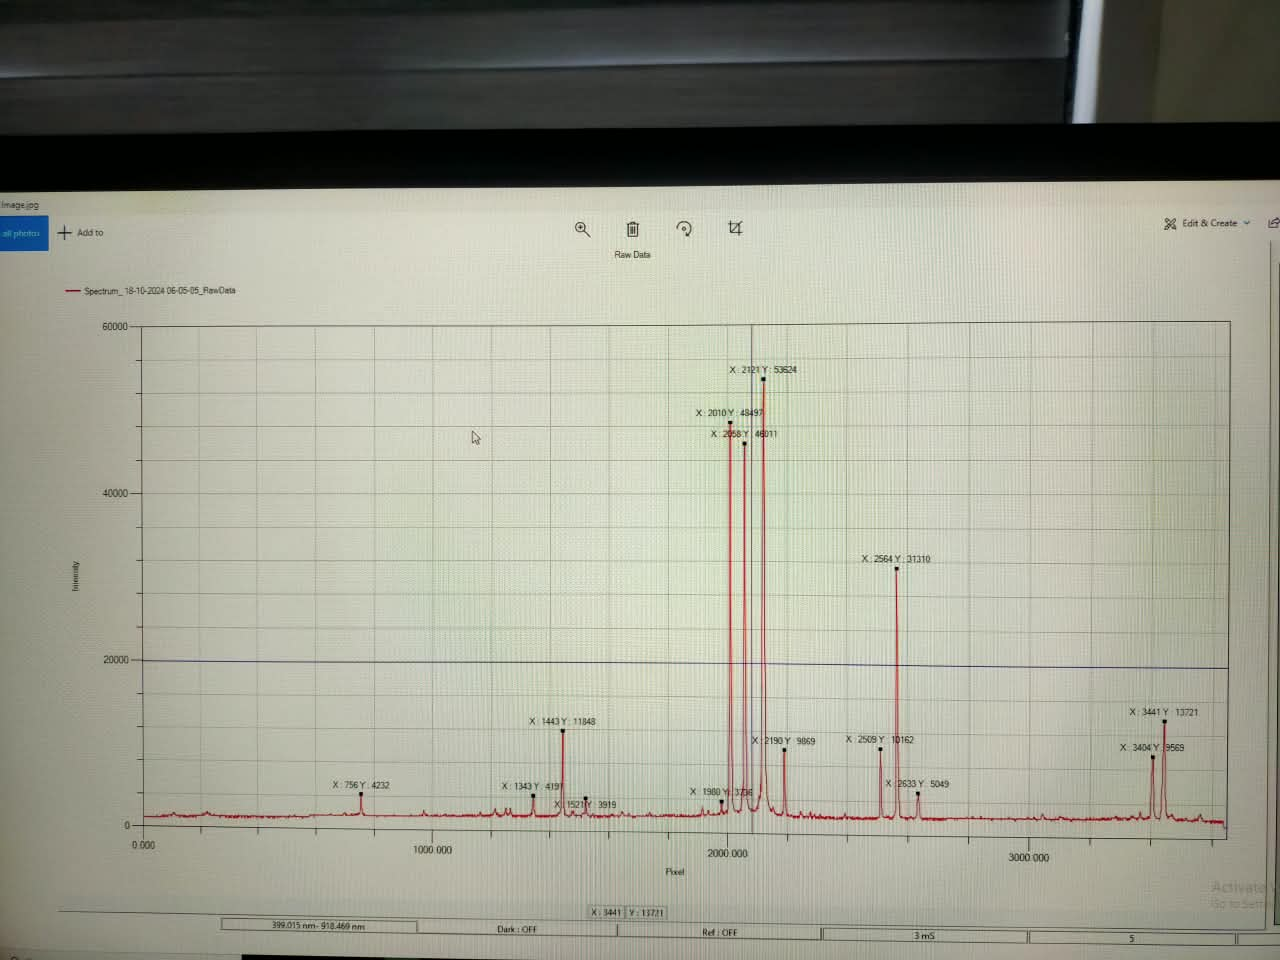
\includegraphics[width=0.95\textwidth]{copper_spectrum.jpeg}
    \caption{Laboratory recorded atomic emission spectrum of the Copper (Cu) arc discharge, displaying prominent green lines in the 510 nm to 522 nm region and blue lines around 465 nm.}
    \label{fig:cu_spec}
\end{figure}

\begin{figure}[H]
    \centering
    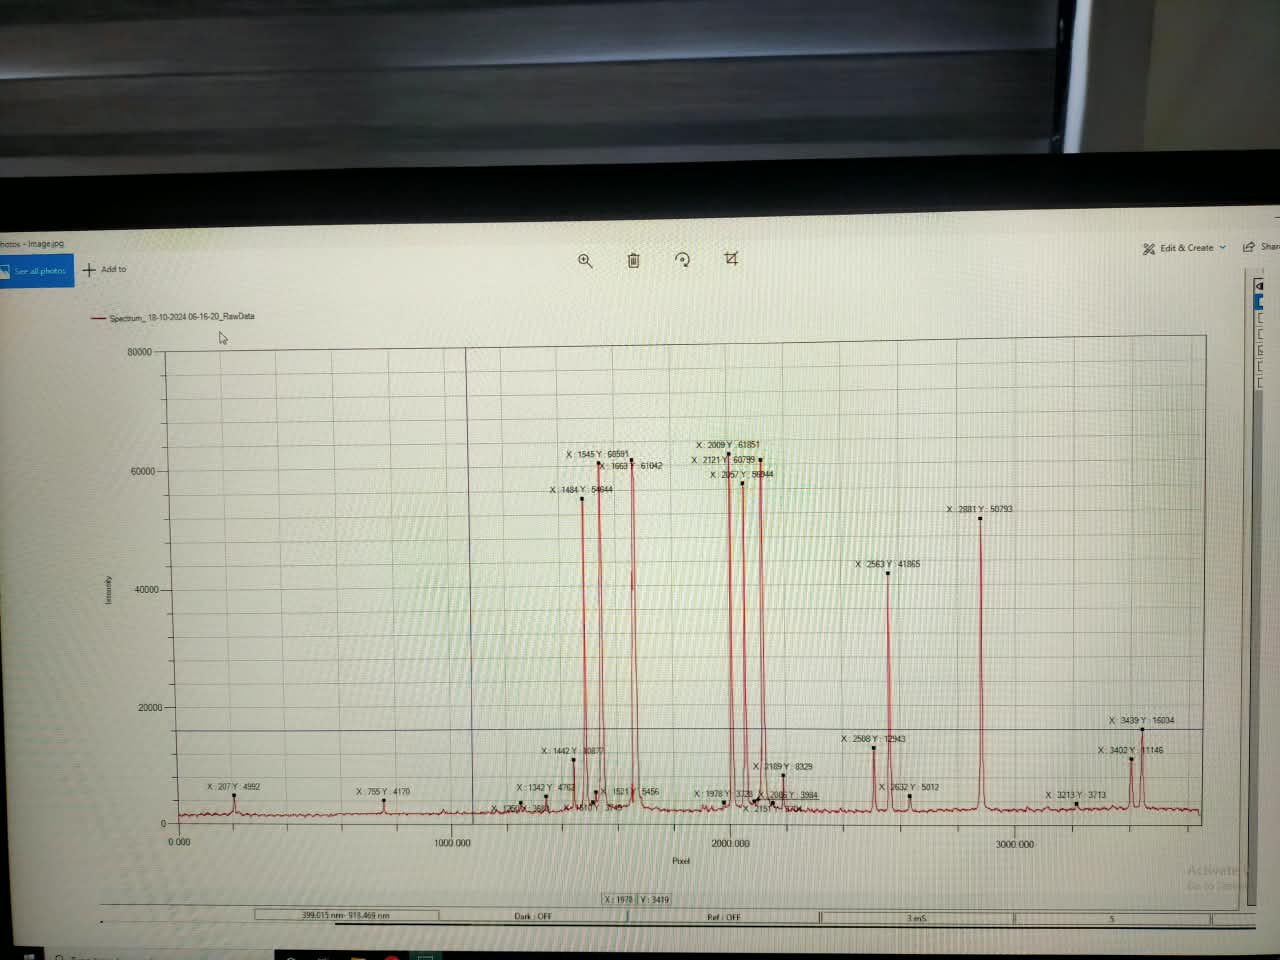
\includegraphics[width=0.95\textwidth]{brass_spectrum.jpeg}
    \caption{Laboratory recorded atomic emission spectrum of the Brass arc discharge, demonstrating the combined spectral signatures of Copper and Zinc, including the distinctive Zinc blue triplet and red emission line.}
    \label{fig:brass_spec}
\end{figure}

\section{Error Calculation}

\subsection{Formula for Percentage Error}
The percentage error for each measured spectral line is calculated using:
\begin{equation}
    \text{Percentage Error} = \left| \frac{\lambda_{\text{calc}} - \lambda_{\text{theo}}}{\lambda_{\text{theo}}} \right| \times 100\%
\end{equation}

\subsection{Summary of Error Analysis}
\begin{itemize}
    \item \textbf{Copper lines:} The maximum percentage error observed was $0.050\%$ (for the 521.641 nm line), and the minimum was $0.007\%$ (for the 578.213 nm line). The mean absolute percentage error across all eight copper lines is $0.027\%$.
    \item \textbf{Brass lines:} The percentage errors for lines attributed to copper in brass averaged $0.023\%$. The errors for zinc lines averaged $0.058\%$, with the largest deviation occurring at the 633.893 nm red line ($0.195\%$).
\end{itemize}

\subsection{Sources of Experimental Error}
\begin{enumerate}
    \item \textbf{Finite Pixel Resolution and Discretisation:} The CCD sensor array has a discrete pixel pitch. The peak position is identified to the nearest pixel integer coordinate. Because the dispersion $\frac{d\lambda}{dd}$ is approximately $0.07\text{ nm/px}$ to $0.21\text{ nm/px}$ depending on wavelength, an uncertainty of $\pm 1$ pixel introduces an inherent wavelength uncertainty of $\pm 0.1\text{ nm}$ to $\pm 0.2\text{ nm}$.
    \item \textbf{Slit Width and Instrumental Broadening:} The entrance slit width is a compromise between optical throughput and resolution. A finite slit width broadens the image of the slit on the detector, leading to instrumental line profiles with finite full-width at half-maximum (FWHM), which slightly affects peak centroid determination.
    \item \textbf{Arc Instability and Thermal Drift:} Electric arcs flicker spatially as the plasma column moves over the electrode tips. Small movements of the arc center can slightly shift the angle of illumination on the entrance slit, causing small apparent wavelength shifts.
    \item \textbf{Dispersion Model Approximations:} While Hartmann's three-parameter relation offers excellent interpolation over visible wavelengths, it is an empirical approximation to the full sellmeier dispersion equation of glass. Higher-order dispersion effects become slightly more pronounced toward the red edge of the spectrum ($> 630\text{ nm}$), which accounts for the slight increase in error observed for the 633.893 nm zinc line.
\end{enumerate}

\section{Discussion}
In this experiment, atomic emission spectroscopy was utilized to study the characteristic spectra of metals and to determine the elemental composition of an unknown alloy. By generating an electric arc between solid metallic electrodes, atoms of the material were thermally vaporised into a plasma column at several thousand Kelvin and excited through energetic electron collisions. When the valence electrons spontaneously decayed to lower energy states, they released discrete photons corresponding to the unique quantised electronic energy levels of the emitting atoms. 

Because the refractive index of optical glass varies non-linearly with wavelength according to Cauchy's dispersion relation, shorter wavelengths experience much greater angular deflection than longer wavelengths. Hartmann's dispersion formula successfully accounted for this non-linear behaviour across the visible spectrum, allowing the CCD pixel coordinates to be mapped accurately to absolute wavelengths using only three calibration lines from a standard low-pressure mercury lamp.

For the pure copper electrodes, the recorded emission peaks closely matched the standard atomic transitions of neutral copper (Cu I), particularly the prominent green triplet in the 510 nm to 522 nm region and blue lines near 465 nm, yielding a mean experimental error of only $0.027\%$. When analyzing the brass specimen, the resulting spectrum exhibited a distinct superposition of atomic emission lines originating from both copper and zinc. In particular, the unmistakable presence of the sharp zinc blue triplet ($468.01\text{ nm}, 472.01\text{ nm}, 481.05\text{ nm}$) and the zinc red transition at $633.89\text{ nm}$ alongside the copper lines confirmed that the specimen is a binary alloy of Copper and Zinc (Brass).

Several notable differences exist between theoretical assumptions and practical laboratory measurements. Theoretically, atomic transitions are modelled as infinitely sharp delta functions with natural linewidths on the order of $10^{-4}$ nm. In real arc discharges, however, emission lines undergo significant physical broadening. High thermal velocities within the hot plasma introduce Doppler broadening, while frequent collisions between emitting atoms, free electrons, and ions cause pressure and Stark broadening. Additionally, the finite width of the entrance slit and the discrete spatial pitch of the CCD array introduce instrumental broadening, giving each observed peak a measurable profile width.

Another practical challenge is the dynamic range of the detector. While theory assumes an ideal linear detector response across all intensities, real CCD arrays experience saturation if integration times are too long, which flattens the tops of strong lines and obscures their true centroid positions. Maintaining a short integration time (3 ms) prevented saturation while preserving faint lines. Furthermore, slight self-absorption in the cooler outer mantle of the arc column and higher-order dispersion deviations at the red end of the spectrum account for minor residual errors, such as the $0.195\%$ error observed for the 633.89 nm zinc line. Overall, the experiment clearly demonstrates the effectiveness of optical emission spectroscopy for qualitative elemental identification and non-destructive alloy verification.

\section{References}
\begin{enumerate}
    \item Jenkins, F. A., and White, H. E. \textit{Fundamentals of Optics}, 4th Edition, McGraw-Hill Education.
    \item Herzberg, G. \textit{Atomic Spectra and Atomic Structure}, Dover Publications.
    \item Kramida, A., Ralchenko, Yu., Reader, J., and NIST ASD Team. \textit{NIST Atomic Spectra Database} (ver. 5.11), National Institute of Standards and Technology, Gaithersburg, MD.
    \item HOLMARC Opto-Mechatronics Pvt. Ltd., \textit{Instruction Manual: CCD Based Constant Deviation Spectrometer for Arc Emission Measurements}.
    \item Kuhn, H. G. \textit{Atomic Spectra}, 2nd Edition, Longmans.
\end{enumerate}

\clearpage
\section{Lab Observations}
The signed laboratory observation sheets from the experiment are attached below:

\begin{figure}[H]
    \centering
    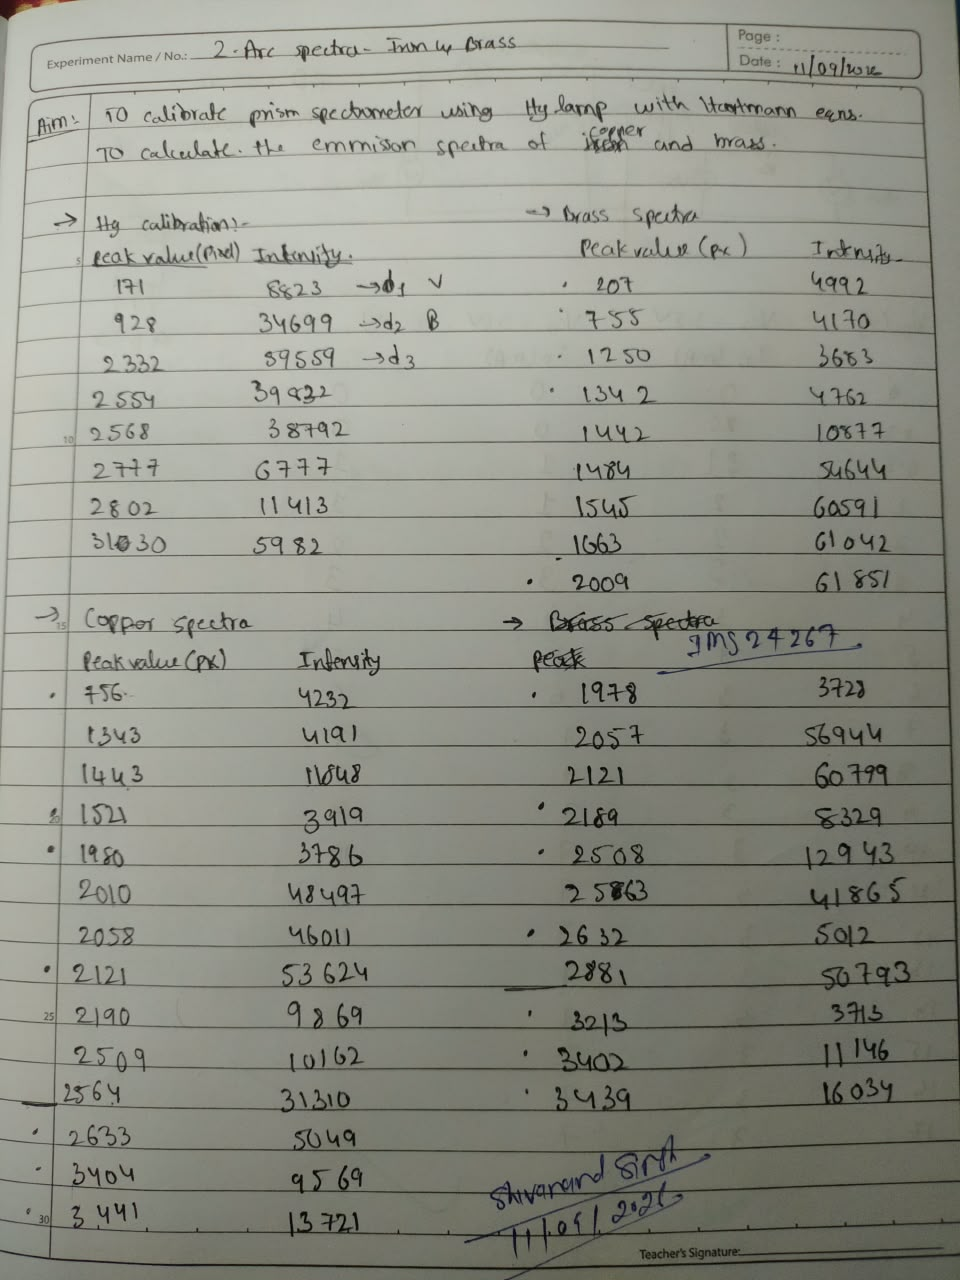
\includegraphics[width=0.70\textwidth]{1.jpeg}
    \caption{Signed raw laboratory observation sheet: Recorded pixel positions and intensities for Mercury (Hg) calibration, Copper (Cu) arc spectrum, and Brass arc spectrum.}
    \label{fig:obs1}
\end{figure}

\clearpage
\begin{figure}[H]
    \centering
    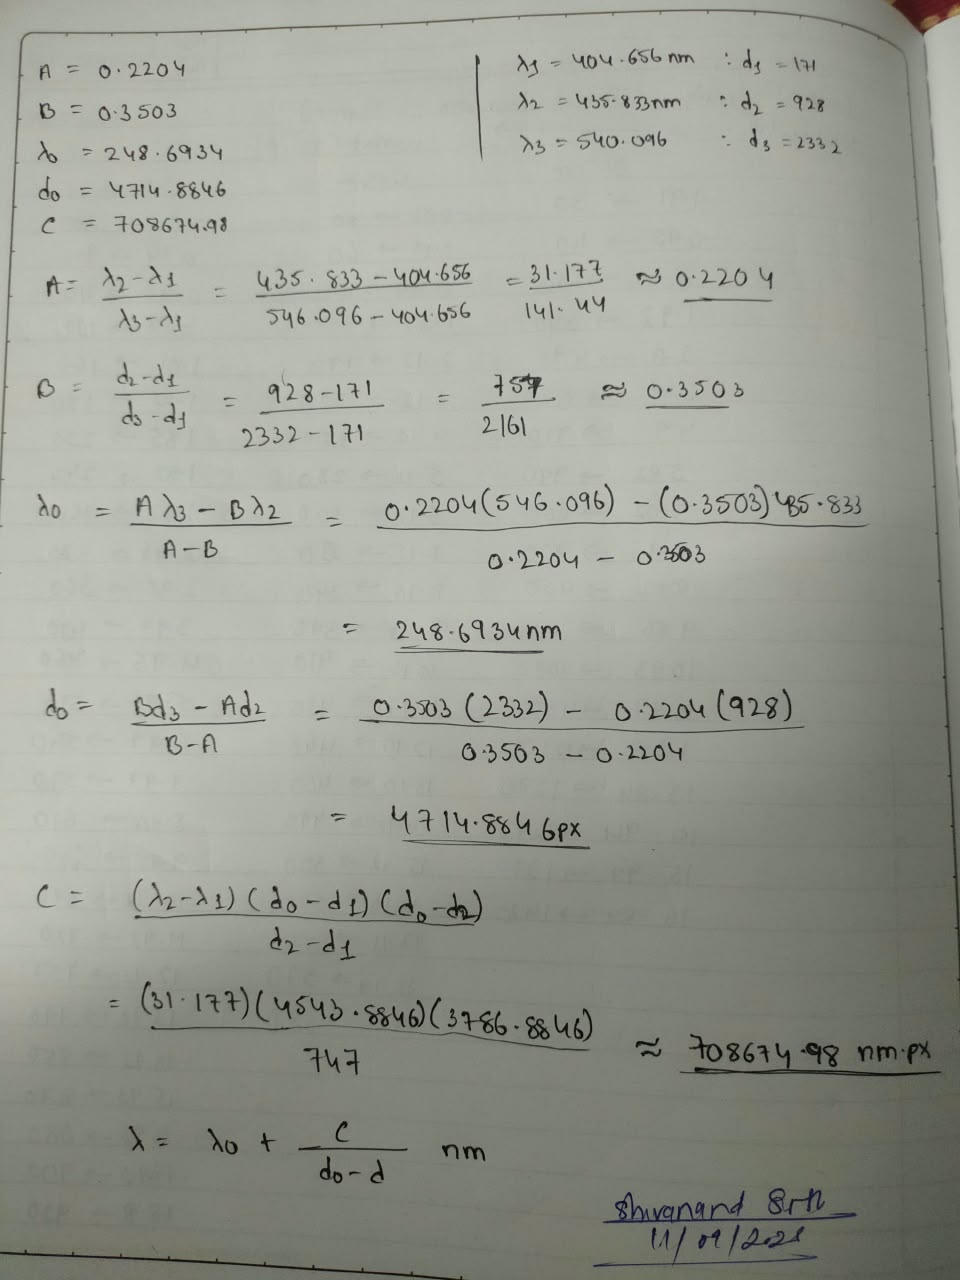
\includegraphics[width=0.80\textwidth]{2.jpeg}
    \caption{Signed laboratory calculation sheet: Step-by-step evaluation of the Hartmann calibration constants $A, B, \lambda_0, d_0,$ and $C$ using standard Mercury emission lines.}
    \label{fig:obs2}
\end{figure}

\end{document}
